\section{Implementation Details}\label{sec:implementation}

\subsection{Switch Model}\label{subsec:model}

\begin{figure}
	%\vspace{-0.1in}
	\centering
		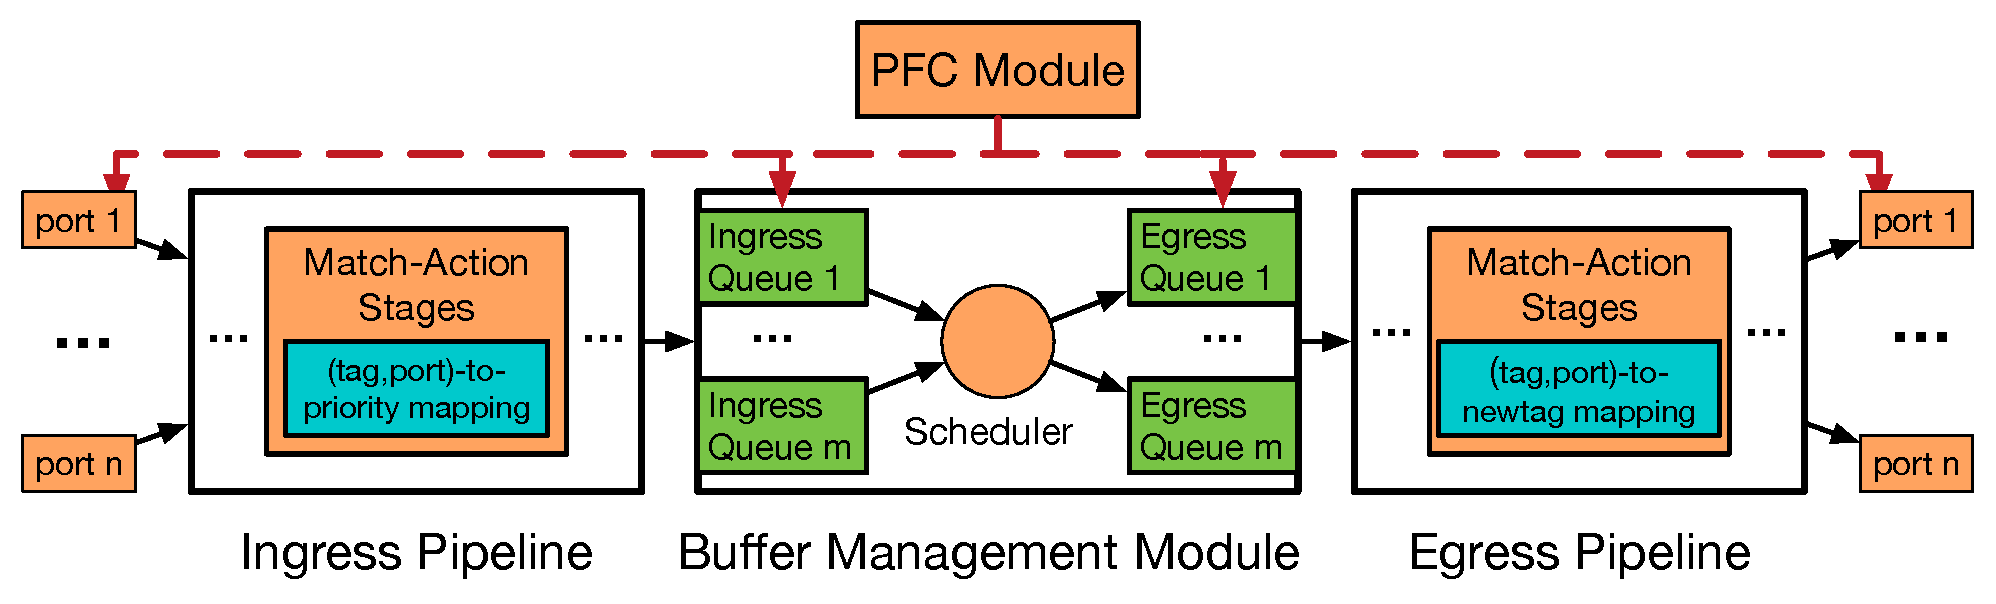
\includegraphics[width=0.5\textwidth] {figs/switch_model}
	\caption{Switch model.}\label{fig:switchmodel}

\end{figure}

In this part, we introduce the switch model on which we implement our algorithm output. As shown in Fig.~\ref{fig:switchmodel},
our switch model consists of five elements: switch port, forwarding engine, PFC engine, crossbar and switch buffer. The function of these elements are list as follows.

%Fig.~\ref{fig:switchmodel}(a) shows the architecture of the switch model, which consists of a switching fabric and N line cards. Line cards are mainly used to receive/send packets and make routing/forwarding decisions. Switching fabric is a module to transfer packet cells from the input line card to the output line card. 

\begin{itemize}
	\item \textbf{Switch port}: The element to receive and send packets. Each switch port consists of an input port and an output port, and is connected with a link.
	
	\item \textbf{Forwarding engine}: The element to make the routing and/or switching decisions. In the forwarding engine, there is a module to decide the priority class of a packet based on the TTL value. 
	
	\item \textbf{PFC engine}: The element to perform PFC function.
	
	\item \textbf{Crossbar}: The element to switch packet cells from the ingress buffer to the egress buffer. 
	
	\item \textbf{Switch buffer}: The element to buffer incoming packets. We assume shared buffer in our model. In the ingress buffer, we use  virtual ingress queue (VIQ) to track the incoming packets. In the egress buffer, we use virtual egress queue (VEQ) to track the outgoing packets. Each VIQ is uniquely corresponding to an input port, while each VEQ is uniquely corresponding to an output port. As shown in Fig.~\ref{fig:switchmodel}, both VIQ and VEQ consist of k queues, with each queue corresponding to a priority class. A packet of priority class $j$ will enter the $j$-$th$ queue of its destined VIQ and VEQ.
	
%    Note that in our switch model, when a packet in some VIQ is forwarded to some VEQ, this VIQ will not perform dequeue operation. Dequeue operation will be performed only after this packet leaves the switch buffer. This is because the purpose of using VIQ is to track the bytes of currently buffered packets received by an input port, such that PFC can work properly.
	
	\textbf{Discussion}: It is not always the case for switch to have both ingress buffer and egress buffer at the same time. It depends on the buffering strategy. If we adopt output-queued strategy, there will be no ingress buffer, and VIQs are simply some counters to record the bytes of buffered packets received by different input ports. If we adopt input-queued strategy~\cite{islip}, there will be no egress buffer, and VEQs can be simulated using virtual output	queuing technique~\cite{tinytera} at the ingress buffer. If we adopt the combined-input-and-output-queued strategy~\cite{chuang1999matching}, the switch will have both ingress buffer and egress buffer. The switching function of crossbar can also be virtual, not necessary to involve packet copying.

\end{itemize}

\textbf{Enqueue and dequeue operations of VIQ and EIQ}: We use $q_{in}^{i}$ to denote VIQ $i$, and $q_{out}^{i}$ to denote VEQ $i$.
Let $q_{in}^{i,j}$ be the $j$-$th$ queue of VIQ $i$, and $q_{out}^{i,j}$ be the $j$-$th$ queue of VEQ $i$ ($1\leq i \leq n$, $1 \leq j \leq k$). The dequeue and enqueue operatons of VIQ and VEQ are performed as follows:
	
	\begin{enumerate}
		\item  Packet $p$ of priority class $j$ enters the switch buffer via input port $i_1$: VIQ $i_1$ performs enqueue operation and puts packet $p$ to the tail of $q_{in}^{i_1,j}$.
		
		\item  Packet $p$ in the head of $q_{in}^{i_1,j}$ is forwarded to VEQ $i_2$:  VEQ $i_2$ performs enqueue operation and puts packet $p$ to the tail of $q_{out}^{i_2,j}$. At the same time, head point of $q_{in}^{i_1,j}$ is moved to the next packet currently queued in $q_{in}^{i_1,j}$. Note that dequeue operation of packet $p$ will not be performed at $q_{in}^{i_1,j}$ at this point in time. 
		
		\item  Packet $p$ in the head of $q_{out}^{i_2,j}$ is forwarded to output port $i_2$: VEQ $i_2$ performs dequeue operation and removes packet $p$ from $q_{out}^{i_2,j}$.  VIQ $i_1$ performs dequeue operation and removes packet $p$ from $q_{in}^{i_1,j}$ (say packet $p$ was previously forwarded from $q_{in}^{i_1,j}$ to $q_{out}^{i_2,j}$). 
	\end{enumerate}
		
	Note that in our switch model, dequeue operation is performed at corresponding VIQ only after packet $p$ leaves the switch buffer. This is because the purpose of using VIQ is to track the bytes of currently buffered packets received by an input port, such that PFC can work properly.

\subsection{Modified PFC Mechanism}\label{subsec:PFC}

As shown in Fig.~\ref{fig:switchmodel}(b), the function of our modified PFC mechanism consists of four parts. 

The PFC engine will track the instant queue lengths of all the VIQs (function (1)). If the queue length of some queue  $q_{in}^{i,j}$ exceeds the configured PFC threshold, PFC engine will generate a PAUSE message to pause the packet transmission of the immediate upstream node on priority class $j$-$1$ over the link connected with port $i$. If the queue length of $q_{in}^{i,j}$ becomes less than the threshold later, PFC engine will generate a RESUME message to resume the packet transmission over the previously paused link on priority class $j$-$1$ (function (2)).

If some output port, say output port $i$, receives a PAUSE or RESUME message on priority class $j$ from its immediate downstream node, the PFC engine will then pause or resume the corresponding egress queue $q_{out}^{i,j}$, accordingly (function (3) and function (4)).

The main difference between our modified PFC mechanism and the typical PFC mechanism is that, if the queue length of some queue $q_{in}^{i,j}$ at some network node exceeds the PFC threshold, PFC engine will pause the packet transmission of the immediate upstream node on priority class $j$-$1$ over the incoming link instead of on priority class $j$. This feature is important for realizing our TTL-based buffer management scheme, as we will introduce in the next.

